%%%%%%%%%%%%%%%%%%%%%%%%%%%%%%%%%%%%%%%%%
% Luca Maurelli CV
%%%%%%%%%%%%%%%%%%%%%%%%%%%%%%%%%%%%%%%%%

%----------------------------------------------------------------------------------------
%	PACKAGES AND OTHER DOCUMENT CONFIGURATIONS
%----------------------------------------------------------------------------------------

\documentclass[10pt]{article}

%\usepackage{showframe}
\usepackage[a4paper,
			includeheadfoot,
			top = 1cm,
			bottom = 0cm,
			left = 1cm,
			right = 1cm]{geometry}

\usepackage{fancyhdr}

% interpreters
\usepackage[utf8]{inputenc}
\usepackage[T1]{fontenc}

% language
\usepackage[english]{babel}
\usepackage{csquotes}

% font
\usepackage{libertine}
\usepackage{courier}

% Paragraph indentation: empty line rather than an indent
\usepackage[parfill]{parskip}

\usepackage{booktabs}
\usepackage{graphicx}

\usepackage{enumitem}
\setlist[enumerate,1]{label=$\vcenter{\hbox{\tiny$\bullet$}}$,leftmargin=*}
\setlist[enumerate,2]{label=--,leftmargin=*}

\usepackage[dvipsnames]{xcolor}
\usepackage[allbordercolors = red,
			colorlinks = true,
            linkcolor = BrickRed,
            urlcolor  = BrickRed,
            citecolor = BrickRed,
            anchorcolor = BrickRed]{hyperref}


\fancyhead[L]{\textit{Luca Maurelli's Curriculum Vitae}}
\fancyhead[C]{}
\fancyhead[R]{\thepage}
\fancyfoot[L]{}
\fancyfoot[C]{}
\fancyfoot[R]{}
\renewcommand{\headrulewidth}{0pt}
\renewcommand{\footrulewidth}{0pt}


\newcommand{\cvsection}[1]{\section*{\centering\normalsize\uppercase{#1}}\vspace{-16pt}\rule{\linewidth}{0.2pt}\vspace{6pt}}

% debug
% \usepackage{showframe}

\begin{document}
% empty header and footer
% https://tex.stackexchange.com/questions/194423/page-style-plain-vs-empty
\pagestyle{empty}

%----------------------------------------------------------------------------------------
%	TITLE PAGE
%----------------------------------------------------------------------------------------
\centering
{\huge\textsc{Luca~Maurelli's~Curriculum~Vitae}\par}
{\textsc{Updated:~}\today\par}
\raggedright
\vspace{1cm}

%----------------------------------------------------------------------------------------
%   PERSONAL DATA
%----------------------------------------------------------------------------------------
\cvsection{personal data}

\noindent
\begin{minipage}[t]{.5\textwidth}
	\raggedright
	\begin{tabular}{@{}ll@{}}
	name surname: & Luca Maurelli\\
	birthdate: & June 30, 1993 \\
	birthplace: & Milan, Italy \\
	phone number: & \href{tel:+393408192088}{(+39)~340~8192088} \\
	e-mail: & \href{mailto:luca.maurelli@unibg.it}{luca.maurelli@unibg.it} \\
	location: & \href{https://goo.gl/maps/qSb6hkSyAdgnEt5w7}{Treviglio~(BG),~24047,~Italy}
	\end{tabular}
\end{minipage}% note the use of "%"
\begin{minipage}[t]{.5\textwidth}
	\raggedleft
	%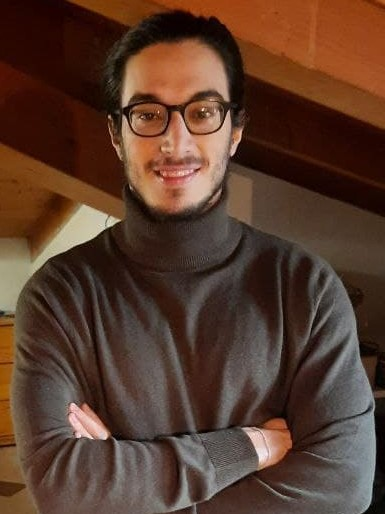
\includegraphics[height=4cm]{face.jpg}
	% ciao ciao \\ 
	% prova \\
	% ciao
\end{minipage}

%----------------------------------------------------------------------------------------
%	ACTUAL WORK EXPERIENCE SECTION
%----------------------------------------------------------------------------------------
\cvsection{current position}

\noindent
\begin{minipage}[t]{.8\textwidth}
	\textbf{Ph.D. Student} at the \href{https://disa.unibg.it/}{Department of Engineering and Applied Sciences} \\
	University of Bergamo
\end{minipage}% note the use of "%"
\hfill\vrule\hfill
\begin{minipage}[t]{.16\textwidth}
	\raggedleft
	Oct 2019 – Present
\end{minipage}

%----------------------------------------------------------------------------------------
%	PREVIOUS WORK EXPERIENCE SECTION
%----------------------------------------------------------------------------------------
\cvsection{previous position}

\noindent
\begin{minipage}[t]{.8\textwidth}
	\raggedright
	\textbf{Research Assistant} at the \href{https://digip.unibg.it/}{Department of Management, Information and Production Engineering}\\
	University of Bergamo
	\vspace{6pt}
	\begin{enumerate}
		\item Project SMART4CPPS, funded by Regione Lombardia, led by 4 OdR and 10 local companies.
		\begin{enumerate}
			\item Management activity of Pilot 1 and Pilot 4
			\item Pilot 1: Design of a health monitoring system for electromechanical actuators (University of Bergamo, Camozzi)
			\item Pilot 4: Machine learning algorithms for the zero-defect end-of-line tuning of medium-voltage switches (University of Bergamo, Cosberg, ABB, CNR)
		\end{enumerate}
		\item Project CRYOABLATION:
		\begin{enumerate}
			\item Model identification of the temperature dynamics in \textit{cryoblation} for atrial fibrillation therapy (Dipartimento di Cardiologia, Ospedale di Seriate)
		\end{enumerate}
		\item Project SP@RK-4.0-I.E.S.:
		\begin{enumerate}
			\item Data analysis and development of a health monitoring and predictive maintenance system in high performance workcenters (Mandelli spa)
		\end{enumerate}
		\item Project SMI-PREDICTIVE MAINTENANCE:
		\begin{enumerate}
			\item Design of a predictive maintenance system for beverage packaging machines using accelerometers (SMI Group)
		\end{enumerate}
  \end{enumerate}
\end{minipage}% note the use of "%"
\hfill\vrule\hfill
\begin{minipage}[t]{.16\textwidth}
	\raggedleft
	May 2018 – Sep 2019
\end{minipage}

%----------------------------------------------------------------------------------------
\vspace{20pt} % Gap between titles
%----------------------------------------------------------------------------------------

\noindent
\begin{minipage}[t]{.8\textwidth}
	\raggedright
	\textbf{Software Engineer} at Consortium Intellimech\\
	\href{https://www.linkedin.com/company/kilometro-rosso/}{Kilometro Rosso}
	\vspace{6pt}
	\begin{enumerate}
		\item Project KNOWLEDGIZE, funded by Regione Lombardia, led by Consortium Intellimech, with 2 OdR and 3 local companies.
		  \begin{enumerate}
			\item Development of a Knowledge Management Web Platform with an Innovative ML Algorithm based on Tag Searching using Django and Google Services (University of Bergamo, University of Brescia, Cosberg, Elettrocablaggi, Vin Service)
		\end{enumerate}
		\item Development of software applications:
		  \begin{enumerate}
			\item Push-bottom panel for testing procedures on PLC in C\#
			\item Monitoring system using industrial communicating protocols MQTT, MTCONNECT, UPC-UA and MODbus in Python
		\end{enumerate}
  \end{enumerate}
\end{minipage}% note the use of "%"
\hfill\vrule\hfill
\begin{minipage}[t]{.16\textwidth}
	\raggedleft
	Oct 2017 – Apr 2018
\end{minipage}

%----------------------------------------------------------------------------------------
%	NEW PAGE
%----------------------------------------------------------------------------------------
\clearpage
\pagestyle{fancy}

%----------------------------------------------------------------------------------------
%	EDUCATION SECTION
%----------------------------------------------------------------------------------------

\cvsection{education}
\textbf{Master's degree in Computer Science}, University of Bergamo, Italy \hfill 110L\slash100 \\
\textit{Development of a Knowledge Management Web Platform with an Innovative ML Algorithm based on Tag Searching} \hfill Mar 2018

%----------------------------------------------------------------------------------------
\vspace{6pt} % Gap between titles
%----------------------------------------------------------------------------------------

\textbf{Bachelor's degree in Computer Science}, University of Bergamo, Italy\hfill 105\slash100 \\
\textit{Development of a library for Mobile Robot Trajectory Control} \hfill Sep 2015

%----------------------------------------------------------------------------------------
%	POST-GRADUATE EDUCATION SECTION
%----------------------------------------------------------------------------------------

\cvsection{post-graduate education}
Ph.D. \textbf{Courses} in:
\begin{itemize}	
	\setlength\itemsep{-6pt}
	\renewcommand\labelitemi{$\vcenter{\hbox{\tiny$\bullet$}}$}

	% https://scholar.google.it/citations?user=nB_7svEAAAAJ
	% https://scholar.google.it/citations?user=-TGDzikAAAAJ
	% https://scholar.google.it/citations?user=rUj9gRgAAAAJ
	% https://scholar.google.it/citations?user=wcXdcwEAAAAJ 
	\item \textit{Nonlinear System Identification} \hfill Politecnico of Milan, Italy\\
	\textbf{Proff. L. Piroddi, S. Formentin, S. Garatti, G. Panzani and L. Fagiano} \hfill 48h, Jan 2019\\
	
	\item \textit{Optimization Models and Algorithms} \hfill University of Bergamo, Italy\\
	\textbf{Prof. M. T. Vespucci} \hfill 24h, Jul 2019\\
	 
	\item \textit{Advanced Mathematical Methods for Engineering} \hfill University of Bergamo, Italy\\
	\textbf{Proff. M. Pedroni and A. Raimondo} \hfill 24h, Oct 2019\\
	 
	\item \textit{Advanced Numerical Methods for Engineering} \hfill University of Bergamo, Italy\\
	\textbf{Prof. C. Vergara} \hfill 20h, Nov 2019\\
	 
	% https://scholar.google.it/citations?user=-h6RUBsAAAAJ

	\item \textit{Noise and Vibration Control Engineering} \hfill University of Brescia, Italy\\
	\textbf{Prof. N. B. Roozen} \hfill 15h, Nov 2019\\
	
	\item \textit{Statistical Signal Processing in Engineering} \hfill Politecnico of Milan, Italy\\
	\textbf{Prof. U. Spagnolini} \hfill 26h, Jan 2020\\
	 
	\item \textit{Numerical Methods for Optimal Control} \hfill IMT School for Advanced Studies Lucca, Italy\\
	\textbf{Prof. M. Zanon} \hfill 30h, May 2020\\
	
	\item \textit{Advanced English Course} \hfill University of Bergamo, Italy\\
	\textbf{Prof. S. J. Kingshott} \hfill 16h, Jun 2020\\
	
	\item \textit{Optimization Models and Algorithms} \hfill University of Bergamo, Italy\\
	\textbf{Prof. M. T. Vespucci} \hfill 15h, Jun 2020\\
	
	\item \textit{Advanced methods for system identification} \hfill University of Bergamo, Italy\\
	\textbf{Prof. M. Mazzoleni} \hfill 20h, Jul 2020\\
	
	\item \textit{Model Predictive Control} \hfill Politecnico of Milan, Italy\\
	\textbf{Proff. M. Farina, R. Scattolini and L. Fagiano} \hfill 26h, Sep 2020\\

	\item \textit{Algorithmic Game Theory} \hfill University of Bergamo, Italy\\
	\textbf{Prof. N. Gatti and Dr. A. Marchesi} \hfill 16h, Oct 2020\\

	\item \textit{Applied Functional Analysis and Machine Learning} \hfill University of Padova, Italy\\
	\textbf{Prof. G. Pillonetto} \hfill 16h, Nov 2020\\

	\item \textit{Applied Linear Algebra} \hfill University of Padova, Italy\\
	\textbf{Prof. L. Schenato} \hfill 16h, Nov 2020\\
\end{itemize}

%----------------------------------------------------------------------------------------
\vspace{6pt} % Gap between titles
%----------------------------------------------------------------------------------------

Ph.D. \textbf{Schools \& Workshops} in:
\begin{itemize}
	\setlength\itemsep{-6pt}
	\renewcommand\labelitemi{$\vcenter{\hbox{\tiny$\bullet$}}$}

	\item \textit{EECI-IGSC 2019 -- Model based Fault Diagnosis using a MATLAB Linear Framework} \hfill University of Padova, Italy\\
	\textbf{Proff. A. Varga and D. Ossmann} \hfill 48h, Mar 2019\\

	\item \textit{Machine Learning: A Computational Intelligence Approach} \hfill University of Genova, Italy\\
	\textbf{Proff. F. Masulli and S. Rovetta} \hfill 20h, Jun 2020\\
	
	\item \textit{RegML 2020 -- Regularization Methods for Machine Learning} \hfill University of Genova, Italy\\
	\textbf{Prof. L. Rosasco} \hfill 20h, Jun 2020\\

	\item \textit{IFAC 2020 -- Set-based Methods in Estimation and Control} \hfill International Federation of Automatic Control (Virtual)\\
	\textbf{Proff. R. Paulen, M. E. Villanueva and B. Chachuat} \hfill 6h, Jul 2020\\

	% \item \textit{EECI-IGSC 2021 -- From Data to Decisions: the Scenario Approach} \hfill International Graduate School on Control (Virtual)\\
	% \textbf{Proff. M. C. Campi and S. Garatti} \hfill 48h, Feb 2021\\

	% \item \textit{EECI-IGSC 2021 -- Learning to Control} \hfill International Graduate School on Control (Virtual)\\
	% \textbf{Prof. S. Formentin} \hfill 48h, May 2021\\

\end{itemize}

%----------------------------------------------------------------------------------------
\vspace{6pt} % Gap between titles
%----------------------------------------------------------------------------------------

%Ph.D. \textbf{Seminars} in: \textit{Optimization and control of airborne wind energy systems}, \textit{Identification for Control}, \textit{Fault diagnosis application in industry and mechatronics}, \textit{Kernel-based learning for system identification}.

Ph.D. \textbf{Seminars} in:
\begin{itemize}
	\setlength\itemsep{-6pt}
	\renewcommand\labelitemi{$\vcenter{\hbox{\tiny$\bullet$}}$}
	\item \textit{Optimization and control of airborne wind energy systems}\\
	\item \textit{Identification for Control}\\
	\item \textit{Fault diagnosis application in industry and mechatronics}\\
	\item \textit{Kernel-based learning for system identification}\\
\end{itemize}

% Ph.D. \textbf{Seminars} in:
% \begin{itemize}
% 	\setlength\itemsep{-3pt}
% 	\renewcommand\labelitemi{$\vcenter{\hbox{\tiny$\bullet$}}$}
% 	\item \textit{Optimization and control of airborne wind energy systems}\\
% 	University of Bergamo, Italy \hfill 2h, Dec 2019\\
% 	\item \textit{Identification for Control}\\
% 	University of Bergamo, Italy \hfill 2h, Nov 2019\\
% 	\item \textit{Fault diagnosis application in industry and mechatronics}\\
% 	University of Bergamo, Italy \hfill 1h, Dec 2019\\
% 	\item \textit{Kernel-based learning for system identification}\\
% 	University of Bergamo, Italy \hfill 1h, Dec 2019\\
% \end{itemize}

%----------------------------------------------------------------------------------------
%	NEW PAGE
%----------------------------------------------------------------------------------------
\clearpage

%----------------------------------------------------------------------------------------
%	TEACHING EXPERIENCE SECTION
%----------------------------------------------------------------------------------------

\cvsection{teaching experience}

\textbf{Lecture Assistant} of the following \textbf{MSc courses} at the University of Bergamo:
\begin{enumerate}
	\setlength\itemsep{-3pt}
	\item \textit{Controlli Automatici} A.Y. 2018/2019 \hfill italian, 20h, Sep – Dec 2018\\
	\item \textit{Controlli Automatici} A.Y. 2019/2020 \hfill italian, 12h, Sep – Dec 2019\\
	\item \textit{Dynamic System Identification} A.Y. 2019/2020 \hfill english, 18h, Jan – Jun 2020\\
	\item \textit{Controlli Automatici} A.Y. 2020/2021 \hfill italian, 12h, Jan – Jun 2021\\
	\item \textit{Identificazione di modelli ed analisi di dati} A.Y. 2020/2021 \hfill italian, 12h, Jan – Jun 2021
\end{enumerate}

%----------------------------------------------------------------------------------------
\vspace{6pt} % Gap between titles
%----------------------------------------------------------------------------------------

\textbf{Co-advisor} of the following \textbf{MSc theses} at the University of Bergamo:
\begin{enumerate}
	\setlength\itemsep{-3pt}
	\item \textit{Sviluppo preliminare di un sistema di health monitoring per un attuatore elettromeccanico}\\
	Advisor: prof. F. Previdi \hfill Students: Davide Palazzini, Alen Preda
	\item \textit{Data-driven health monitoring di attuatori elettromeccanici per automazione industriale}\\
	Advisor: prof. F. Previdi \hfill Students: Davide Presciani, Matteo Gusmini
	\item \textit{Simulatore elettro-termo-meccanico di strisce bimetalliche per interruttori industriali a bassa tensione}\\
	Advisor: prof. F. Previdi \hfill Student: Paolo Pasinetti
	\item \textit{Predizione della vita utile residua di valvole elettropneumatiche usando tecniche di machine learning}\\
	Advisor: prof. F. Previdi \hfill Student: Angela Pomata
\end{enumerate}

%----------------------------------------------------------------------------------------
%	PUBLICATIONS SECTION
%----------------------------------------------------------------------------------------

\cvsection{publications}

\textbf{International conferences}
\begin{enumerate}[label={[C0{\arabic*}]}]
	\setlength\itemsep{-3pt}
	\item M. Mazzoleni, M. Scandella, \textsc{L. Maurelli}, F. Previdi.\\
	\textit{Mechatronics applications of condition monitoring using a statistical change detection method.}\\
	Accepted for publication to 21st IFAC World Congress, Berlin, Germany, July 12-17, 2020
	\item \textsc{L. Maurelli}, M. Mazzoleni, F. Previdi.\\
	\textit{Modeling and simulation of bimetallic strips in industrial circuit breakers.}\\
	Submitted to 19th IFAC Symposium on System Identification, (Virtual) Padova, Italy, July 14-16, 2021
\end{enumerate}


\vfill
{\centering \textbf{Waiver} \par}
I authorize the treatment of my personal data in compliance with the Italian Legislative Decree 196/2003 and the article GDPR 679/16 - “European regulation on the protection of personal data”

\end{document}
